\chapter{Proposed Architecture}
\label{ch:arch}
The architecture design is targeted to capture as much data reuse opportunity as possible, a three-level hierarchy on-chip buffer exploits almost every data reuseability in a regular convolution layer in the mean time saving power by logistically decreasing buffer size: data stays longer in the lower and smaller hierarchy buffer. As parallelism goes up, dispatching memory to each PE becomes a huge burden to the control logic; with data rearrangement, we can efficiently transfer data between buffer and buffer, or buffer and PE with shifter instead of MUX, saving logic and potentially power. We propose three micro-architecture dedicated to low-bit multiplication adder tree, able to operate on 1,2,4,8 bits signed and unsigned data, and an additional XNOR functionality. Finally a 5-stage pipeline PE structure is proposed to process \textit{output row stationary} convolution.
Power consumption is usually the bigger concern before performance when it comes to deploying DNN onto mobile devices. It has been shown that the main source of energy consumption comes from memory access from buffers and off-chip memory \cite{EIE}\cite{Eyeriss}. In comparison to memory access from register file or simple arithmetic operations, memory access to several dozen KB of SRAM uses an order of magnitude more energy, and yet off-chip memory access from DRAM takes as much as  three orders of magnitude more energy. This sets our goal straight to have the data stay at lower energy consumption unit as longer as possible.

\section{System Overview}
\autoref{fig:architecture} shows the top-level architecture and memory hierarchy of the proposed system. The system consists of a 16x16 PE array, 100KB global single-port SRAM buffer, a column of size 16 of single-port 8KB weight buffer, a row of size 16 of single-port 16KB input buffer, a 1D PE taking care of post-processing. With careful data axis re-alignment, module-to-module data requires at most a shift from bank to bank without costly MUX. A PE column processes in lock-step, passing finished partial sum to neighbor PE column on their right until the edge of PE array, getting rid of complex routing logic needs for collecting data from PE array to global buffer. Input and Weight buffer broadcast their data to PE array along column and row respectively, similar to \cite{PrecisionScalableVLSI}\cite{ENVISION}, once again requires no costly \textit{network-on-chip} routing data as \cite{Eyeriss} does. Each PE takes rows of data each time, producing one row of output partial sums, capturing every convolutional reuse opportunities in its register files and partial sum register; inherited from \cite{Eyeriss} naming convention, we call this \textit{output row stationary}.  
\begin{figure}
    \centering
    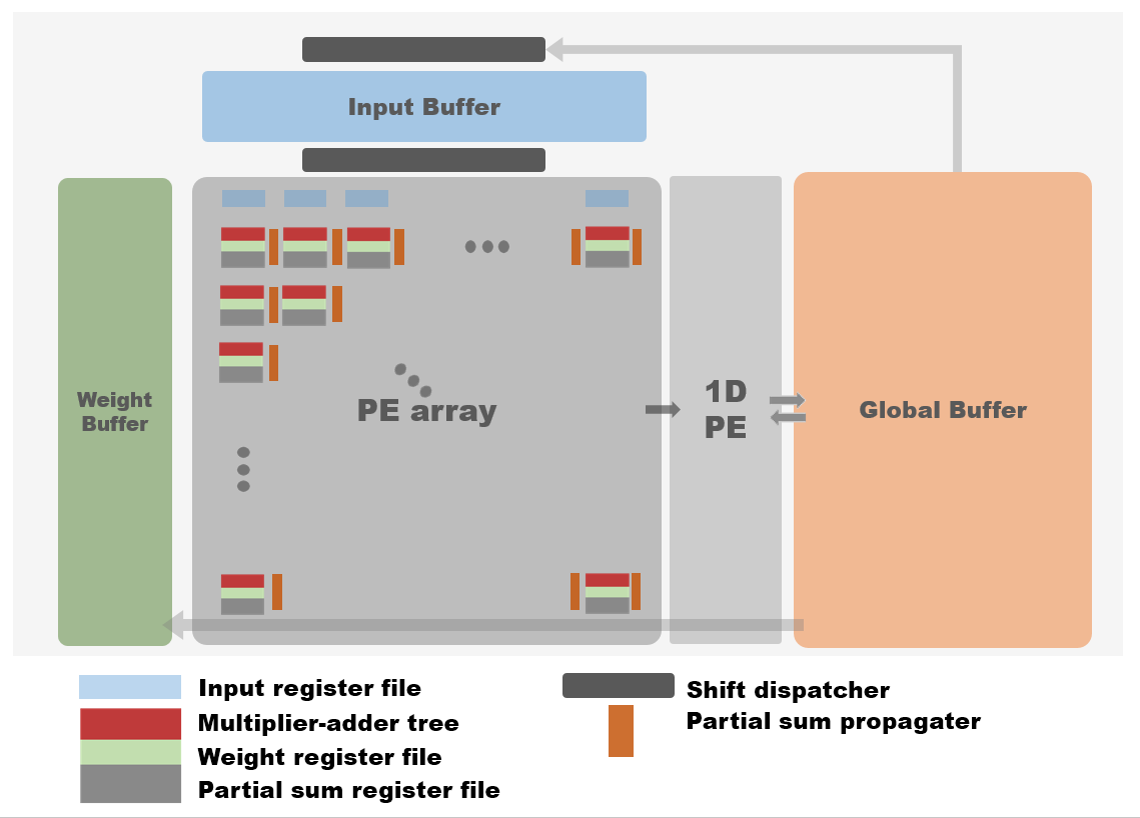
\includegraphics[width=0.8\linewidth]{inc/4_proposed_architecture/figure/architecture.png}
    \caption{System architecture.}
    \label{fig:architecture}
\end{figure}



\subsection{Dataflow}
\begin{figure}[h]
    \centering
    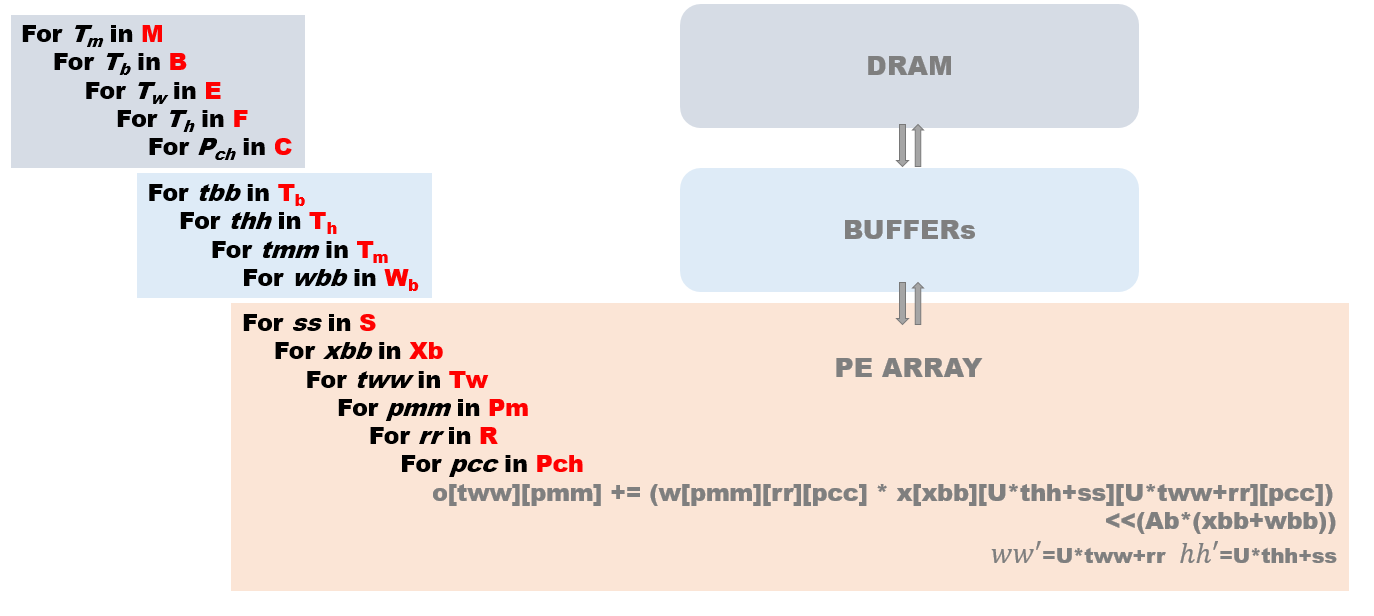
\includegraphics[width=1\linewidth]{inc/4_proposed_architecture/figure/dataflow.png}
    \caption{An overview of the proposed dataflow.}
    \label{fig:dataflow}
\end{figure}
\begin{figure}[h]
    \centering
    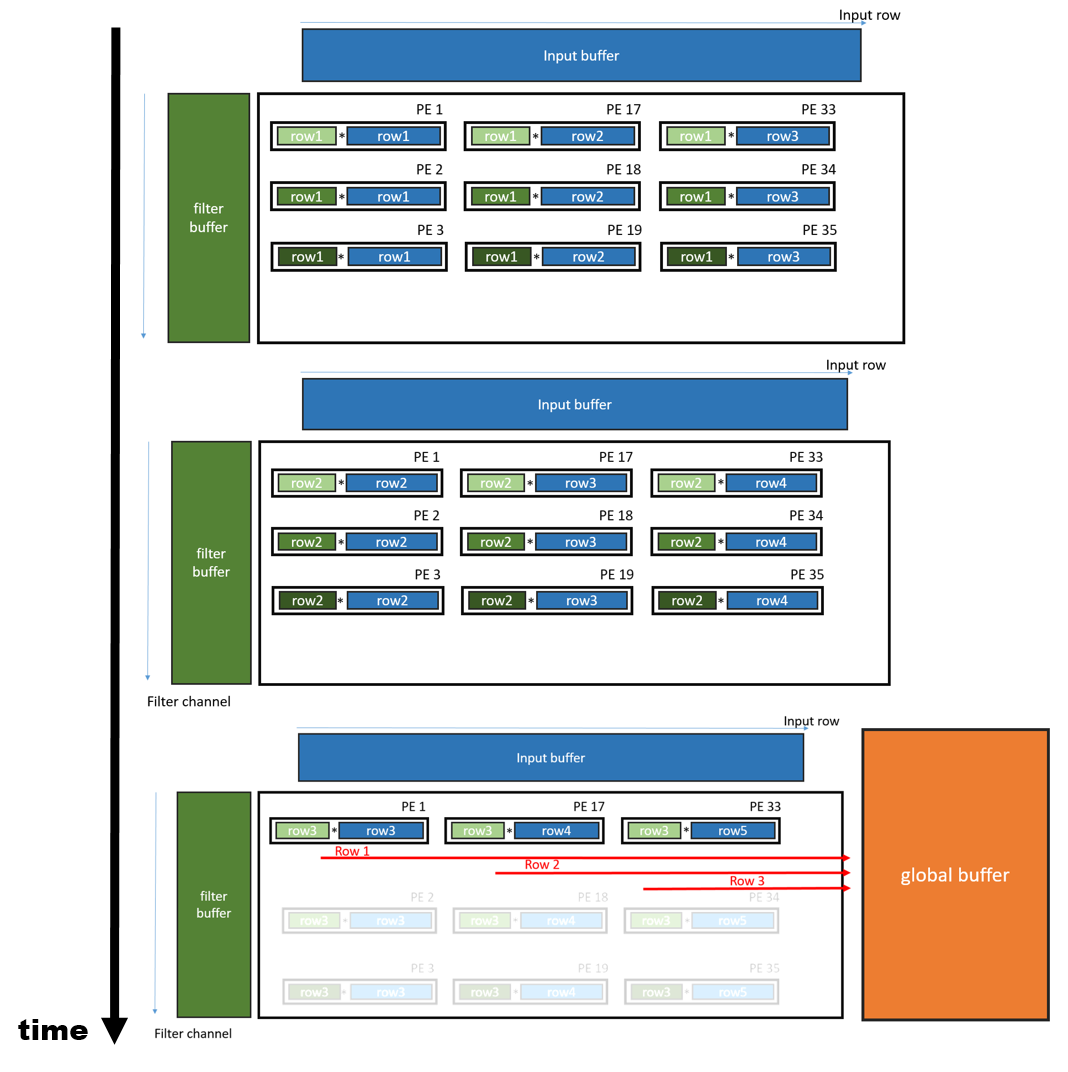
\includegraphics[width=1\linewidth]{inc/4_proposed_architecture/figure/pe_dataflow.png}
    \caption{PE performing 1D convolution on a partial sum row.}
    \label{fig:pe_dataflow}
\end{figure}
\autoref{fig:dataflow} shows the outlook on the dataflow of one layer of CNN on our architecture, definitions of some looping factors can be found in the following sections. The figure gives an idea of data reuse opportunity spread through three level of memory hierarchy of off-chip DRAM, on-chip SRAM buffer, and register files inside each PE. Each PE is in charge of one output partial sum row and computes 1D convolution over a number of dimension; as soon as the computation is done, the output row written to the global buffer is never accessed again before switching to the next input channel tile, reusing data at its best in other word. The input and weight buffer reuse the data \textit{spatially row-wise}, each data in the both buffer will be accessed at least $\boldsymbol{S}$ times. The trickier part lies in the input row data reuse, we spread input rows across input buffer banks based on stride $\boldsymbol{U}$, with a simple shift, each column of PE can gain access to the data every cycle, granting the best bandwidth input buffer can offer, at the same time reuse data along $\boldsymbol{S}$ dimension. Further but relatively rare reuses include input data along $\boldsymbol{W_b}$ dimension, weight data along $\boldsymbol{T_h}$ or/and $\boldsymbol{T_b}$ dimensions.  \\
The permutation of the for loops has a heavy impact on the data re-usability out of PE loops. Since the buffer size is limited, the deeper nested the loop is, the frequent the data has to be thrashed, once this happens, the re-usability in the upper loops is forfeited. Therefore for loops in blue blocks in \autoref{fig:dataflow}, we arrange looping dimension as deeper as more likely the index to be 1. \\
\autoref{fig:pe_dataflow} demostrates the \textbf{\textit{output row stationary}} dataflow where each PE keeps an partial sum row stationary, taking rows of input and weight from buffers and perform 1D convolution, and output the partial sum through the partial sum propagator out of the PE array to global buffer or off-chip. 
\subsection{Data tiling}
Data tiling is widely used in the computation of large matrix-matrix multiplication, and is necessary for NN application. \autoref{fig:tiling} gives an overview of the four tiling parameters we use. The gray dotted line enclosed cubes are the data we would pass to the processor at each iteration. $P_{ch},P_m$ are the channel size and filter size processed by PE at a time. \\
\begin{figure}[h]
    \centering
    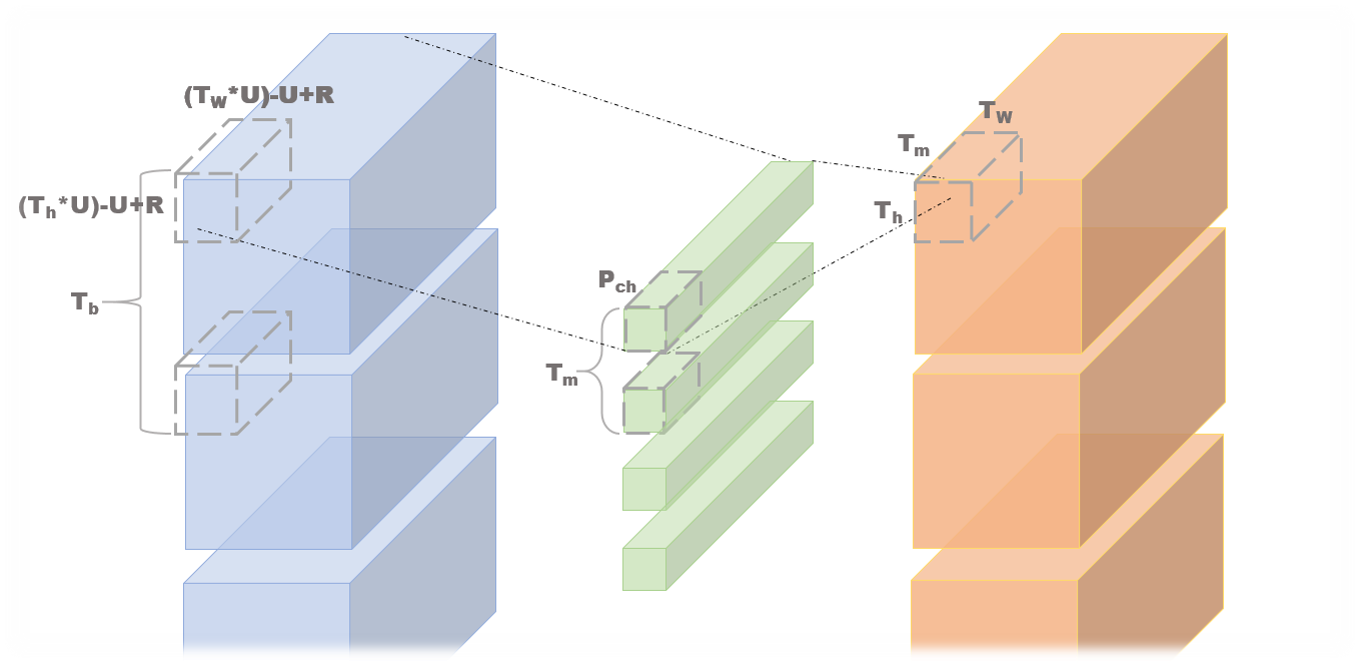
\includegraphics[width=1\linewidth]{inc/4_proposed_architecture/figure/tiling.png}
    \caption{Tiling parameters on tensors.}
    \label{fig:tiling}
\end{figure}

\begin{table}[h]
    \caption{Tiling shape parameters}
    \label{tab:tile_shape}
    \centering
    \footnotesize 
        \begin{tabular}{cc}
        \toprule
        Parameter & Description \\
        \midrule
            $T_m$ & filters\\
            $T_w$ & feature map Width tile\\
            $T_h$ & feature map Height tile\\
            $T_b$ & Batch tile\\
        \bottomrule
        \end{tabular}
\end{table}
\begin{figure}[h]
    \centering
    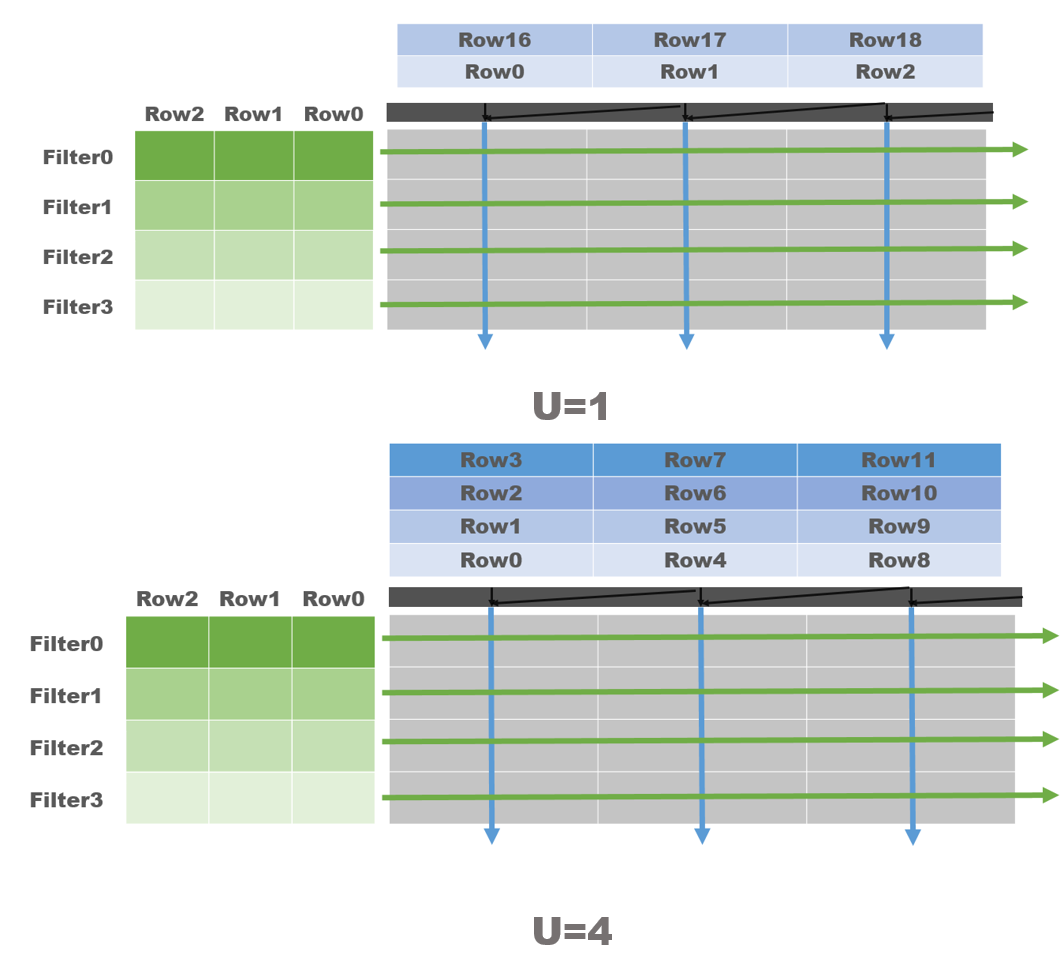
\includegraphics[width=1\linewidth]{inc/4_proposed_architecture/figure/stride_buffer.png}
    \caption{Input and Weight buffer data arrangement and their relation with stride $U$.}
    \label{fig:stride_buffer}
\end{figure}
\subsection{Data re-alignment and buffer hierarchy}
The data is specially arranged in the following manners \autoref{tab:addr_map} in global buffer. The global buffer is a 32-banks single-port SRAMs arranged in 2 groups, providing maximum 32x32b bandwidth per cycle.  This packs the data in a way the data can be access from all the banks without bank conflict, granting maximum bandwidth. The tensors are viewed as collections of \textit{row tensors}, couple with indexes to the rows for data re-alignment purpose. First the tensors are re-arranged as multi-dimensional array of \textit{row tensor} and \textit{row index tensor} parts, the group and bank are chosen based on the flattened tensor index, and compact row tensors accordingly in a buffer bank. \\
\autoref{fig:filter_arrange} shows how the filter tile $T_m$ is split-ed based on $P_m$, in order for the output quantization module packs contagious channels together, therefore saving off-chip memory access. This is the main contribution of this work, with the constraint of multiples of 16 filters computed by 16 PE rows in lock-step, so the output can be quantized and re-packed online. Input and Weight bank counts matches the PE array dimensions, so the data is accessed from each banks in one cycle, and broadcast-ed to PE columns or rows. \\
\autoref{fig:stride_buffer} shows how data would be arranged in input and weight buffers. For input data specially, they are spread-ed across banks based on stride $U$, so the PE array can have required data with only a single shift from the output of input buffer. For example for 11x11 convolution with stride 4, the first output row takes \textbf{Row0} to \textbf{Row10}, the second output row takes \textbf{Row4} to  \textbf{Row14}, at the first row iteration, \textbf{Row0 Row4} can be accessed simultaneously, at the last row iteration, \textbf{Row10 Row14} can be accessed simultaneously with a left-shift of 2, operated by the shifter dispatcher in black box between PE array and input buffer. \\
\begin{table}[h]
    \caption{Global buffer address space mapping}
    \label{tab:addr_map}
    \centering
    \footnotesize 
        \begin{tabular}{cccc}
        \toprule
        Row tensor & Row index tensor & bank & group \\
        \midrule
            $\boldsymbol{I_r}[X_b][W'][P_{ch}]$ & $\boldsymbol{I_{idx}}[T_b][H']$  &$\boldsymbol{I_{idx}.flatten}\%16$ & $\boldsymbol{I_{row}.flatten}\%2$\\
            $\boldsymbol{W_r}[S][R][P_m]$ & $\boldsymbol{W_{idx}}[\lfloor T_m/P_m \rfloor][W_b]$     
            & $\boldsymbol{W_{idx}.flatten}\%16$ & $\boldsymbol{W_{row}.flatten}\%2$\\
            $\boldsymbol{O_r}[T_w][P_m]$ & $\boldsymbol{O_{idx}}[\lfloor T_m/P_m \rfloor][T_b][T_h]$ 
            & $\boldsymbol{O_{idx}.flatten}\%16$ & $\boldsymbol{O_{row}.flatten}\%2$\\

        \bottomrule
        \multicolumn{4}{c}{$H'=(T_h*U)-U+R\quad W'=(T_w*U)-U+R$} 
        \end{tabular}
\end{table}
\begin{figure}[h]
    \centering
    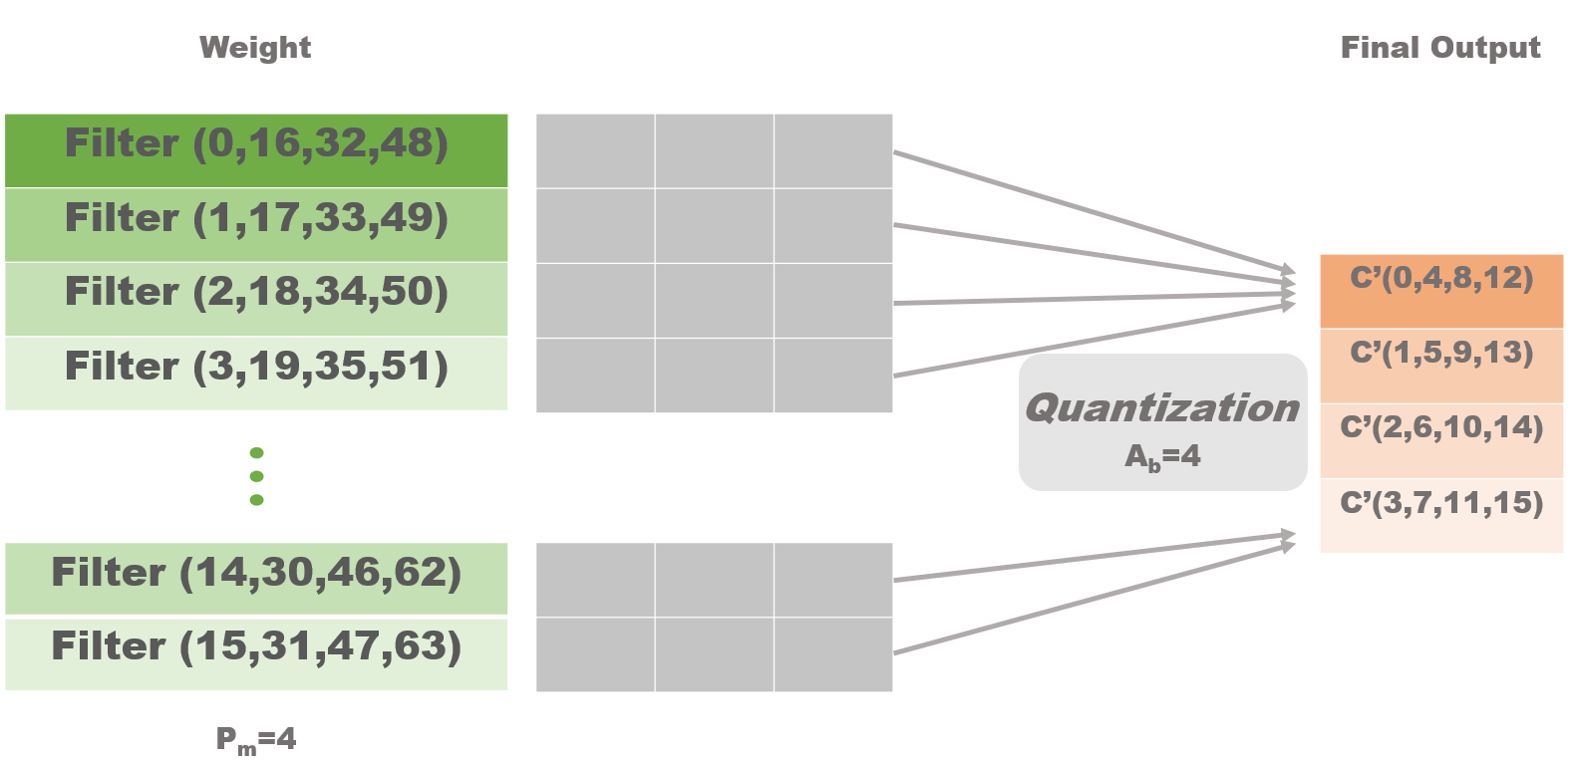
\includegraphics[width=1\linewidth]{inc/4_proposed_architecture/figure/filter_arrange.png}
    \caption{Filter index re-arranged based on $P_m$, so the output can be quantized and re-packed sequentially channel-wise.}
    \label{fig:filter_arrange}
\end{figure}

\autoref{tab:buffer_spec} shows the specifications of the three data buffers. The parameters are mainly chosen based on worst case CNN shape parameter. The constrains are given by \autoref{tab:buffer_cons}. Input buffer size is chosen based on \textbf{AlexNet} \textit{conv1} layer with $W'=63,P_{ch}=1,X_b=2,U=4$. Weight buffer size is chosen based on \textbf{AlexNet} \textit{conv1} layer with $R=S=11,P_m=2,P_{ch}=1$. Global buffer size is chosen with based on \textbf{AlexNet} \textit{conv1} layer with a set of processing parameters to be of 100KB, the configuration will be provided in \autoref{ch:results}. 
\begin{table}[h] 
    \caption{Buffer specifications}
    \label{tab:buffer_spec}
    \centering
    \footnotesize 
        \begin{tabular}{c|cccc}
        \toprule
        Buffer  & banks & size & width & total size \\
        \midrule
        Input & 16 & 512 & 16 & 16KB\\
        Weight & 16 & 256 & 16 & 8KB\\
        Global & 32 & 800 & 32 & 100KB\\
        \bottomrule
        \end{tabular}
\end{table}
\begin{table}[h]
    \caption{Buffer constraints}
    \label{tab:buffer_cons}
    \centering
    \footnotesize 
        \begin{tabular}{c|c}
        \toprule
        Buffer &  constraints\\
        \midrule
        Input & $W'*P_{ch}*X_b*U \leq 512$\\
        Weight & $R*S*P_m \leq 256$\\
        Global & $Input+Weight+Partial\ sum\ size \leq 100KB$ \\
        \midrule
        \multicolumn{2}{c}{$Input\ size= H'*W'*P_{ch}*X_b*T_b$}\\
        \multicolumn{2}{c}{$Weight\ size= T_m*S*R*W_b*P_{ch}$}\\
        \multicolumn{2}{c}{$Partial\ sum\ size =T_b*T_m*T_h*T_w*psum\ width$}\\
        \bottomrule
        \multicolumn{2}{c}{psum width is either 16/32 bits}
        \end{tabular}
\end{table}
\section{Architecture}
\subsection{PE processing pipeline}
\begin{figure}[h]
    \centering
    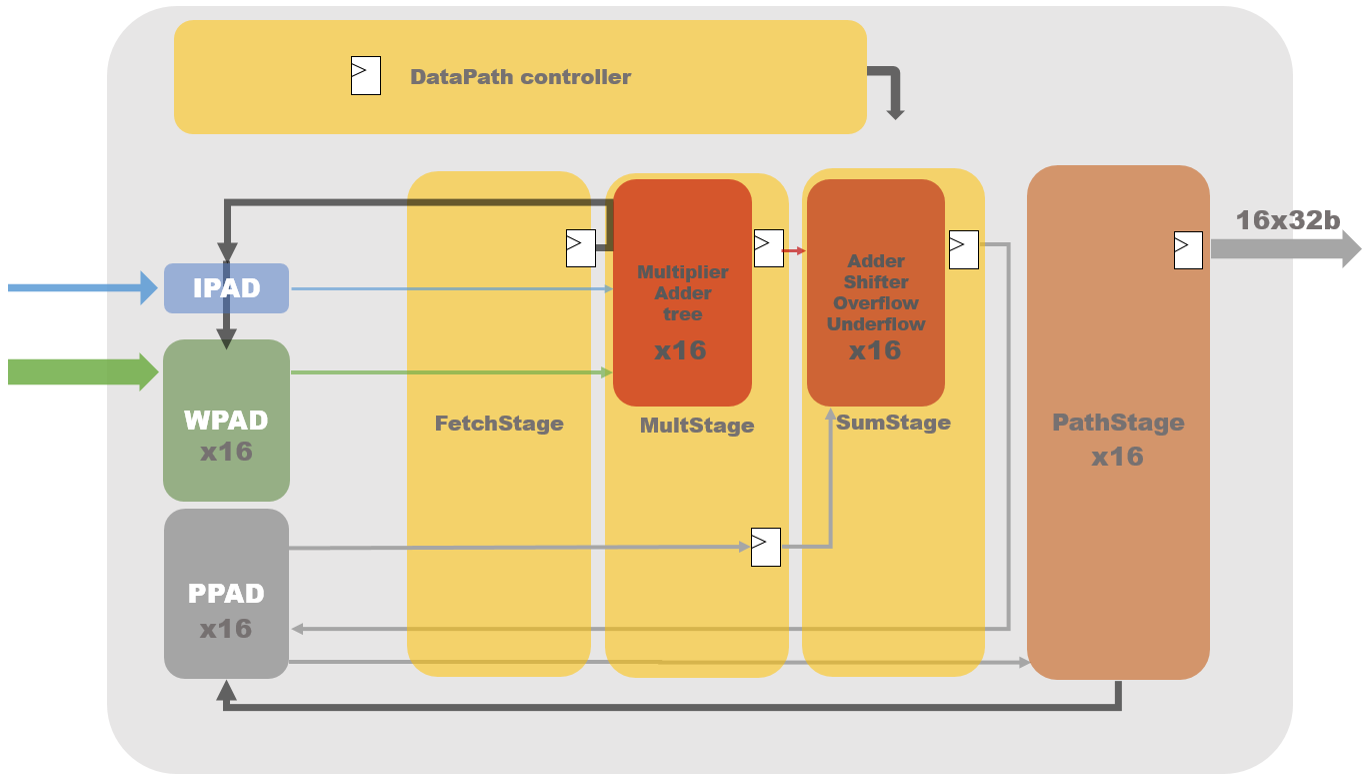
\includegraphics[width=1\linewidth]{inc/4_proposed_architecture/figure/PE.png}
    \caption{PE column pipeline.}
    \label{fig:pe}
\end{figure}
PE consist of a 3-stage processing pipeline, three register-files holding input, weight and partial sum, and a partial sum propagate pipeline. The first stage is the \textit{Fetch stage}, its serves solely as a delay unit for register file data read. The second stage is the main contribution of this work, the \textit{Multiplication stage} consisting of multiplier-adder trees that multiplies and add two 16-bit data subword-ly. The third stage \textit{summation stage} is made of a 32-18 bit signed adder and a shifter. The adder can be configured to be a 16-16 bit signed adder for 16-bit partial sum. The shifter left shift the data $A_b*(wbb+xbb)$ bits, matching the data weighting according to the current bit-channels. The summation operation saturates any overflow or underflow data. The partial sum stays in the partial sum register in this stage for $P_{ch}*R$ cycles, and then written to \textit{PPAD}, the partial sum register file. \\
The final stage \textit{output propagate path stage} works as a FIFO, it takes partial sum from neighbor PE on its left or read from the PPAD, and passes the partial sum down the propagate path to its neighbor PE on the right. The stage chooses its partial sum source in a round-robin manner, if both partial sums from left PE and PPAD are available, it takes the source other than the last source processed. The propagate path throughput is 16x32bit, it has to sends out $\textit{Active PE row}*P_m*T_w$ number of data before the new partial sum row being processed overlaps the PPAD address without any latency. The overlapping condition is $16*P_m*T_w \geq R*P_{ch}*2*T_w*P_m$ , which means that the PE can't generates two rows of partial sum with the cycles it takes to transfer 16 rows of partial sum out of the PE array without stalling the PE processing, 16 is the worst case where every PE columns are active. In practice, even the unwanted latency presents, it doesn't deter the entire processing much as a partial sum are sent out every $R*S*P_{ch}*T_w*P_m*X_b$ cycles, the latency would always be negligible. As we can see the condition is always met for fixed PE array dimension, it limits the scalability of the architecture, the column number can't be too big for global buffer bandwidth to bear. \\
Now to the data \textit{scratch pad}. Every PE is equipped with one of each input, weight and partial sum scratch pad. The scratch pads are register files that hold data for the purpose of convolutional data reuse. The scratch pad specifications and constraints are given by \autoref{tab:pad_spec} and \autoref{tab:pad_cons}. The input and weight pad hold a window of current 1D convolution window, the partial sum pad instead holds $P_m$ rows of partial sum. Note that the partial sum PAD is a 32x32b register file, capable of handling both 16-bit and 32-bit partial sum data. Practically configuration larger than 8-bit and 4-bit input and weight requires 32-bit partial sum to prevent constant overflow or underflow, yet a 4-bit to 4-bit setting, which consists most portion of our best \textbf{AlexNet} model, 16-bit partial sum is enough. With knowledge of scratch pads, we provide an example in \autoref{fig:tww} and \autoref{fig:xb_to_s} demonstrating the data storage in pads and 1D convolution dataflow in terms of looping indexes. \\
\begin{figure}
    \centering
    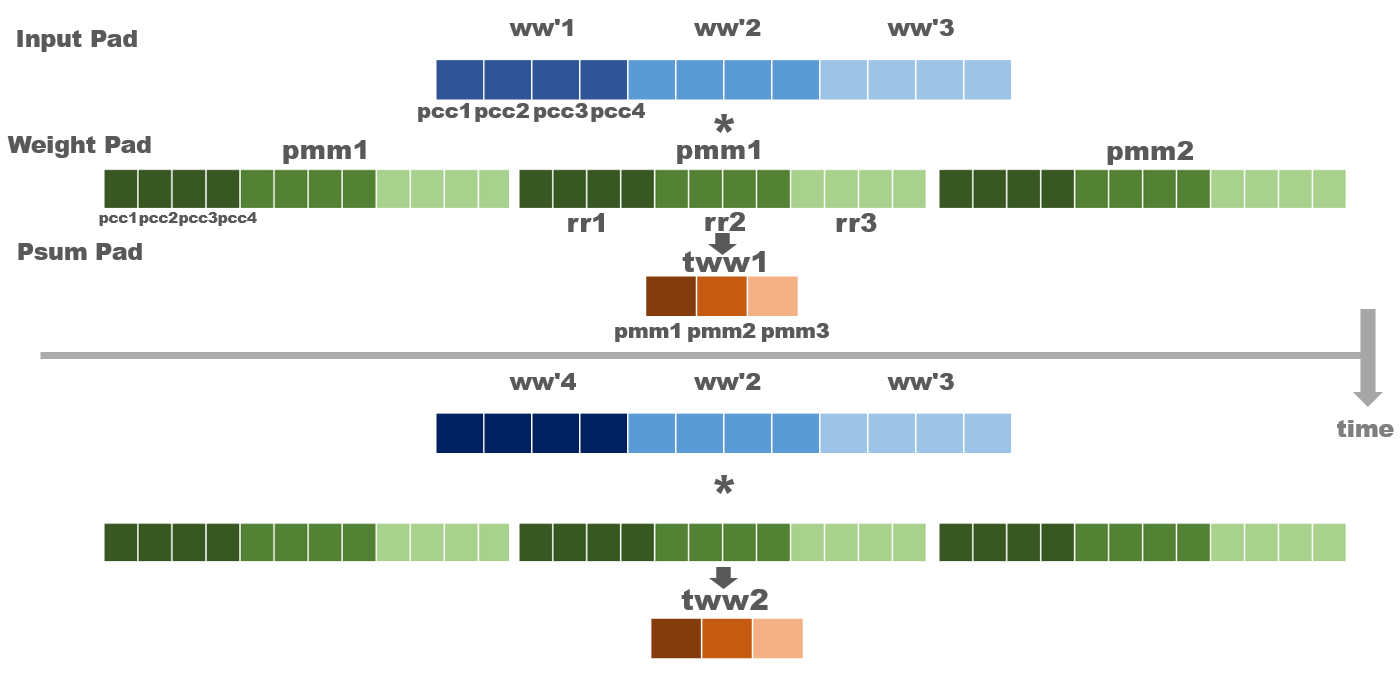
\includegraphics[width=1\linewidth]{inc/4_proposed_architecture/figure/tww.png}
    \caption{An example of 1D convolution with $P_{ch}=4,P_m=3$, at finishing first partial sum pixel tww1, input pixel ww'1 is replaced in input pad with ww'4, and proceed to partial sum pixel tww2. }
    \label{fig:tww}
\end{figure}
\begin{figure}
    \centering
    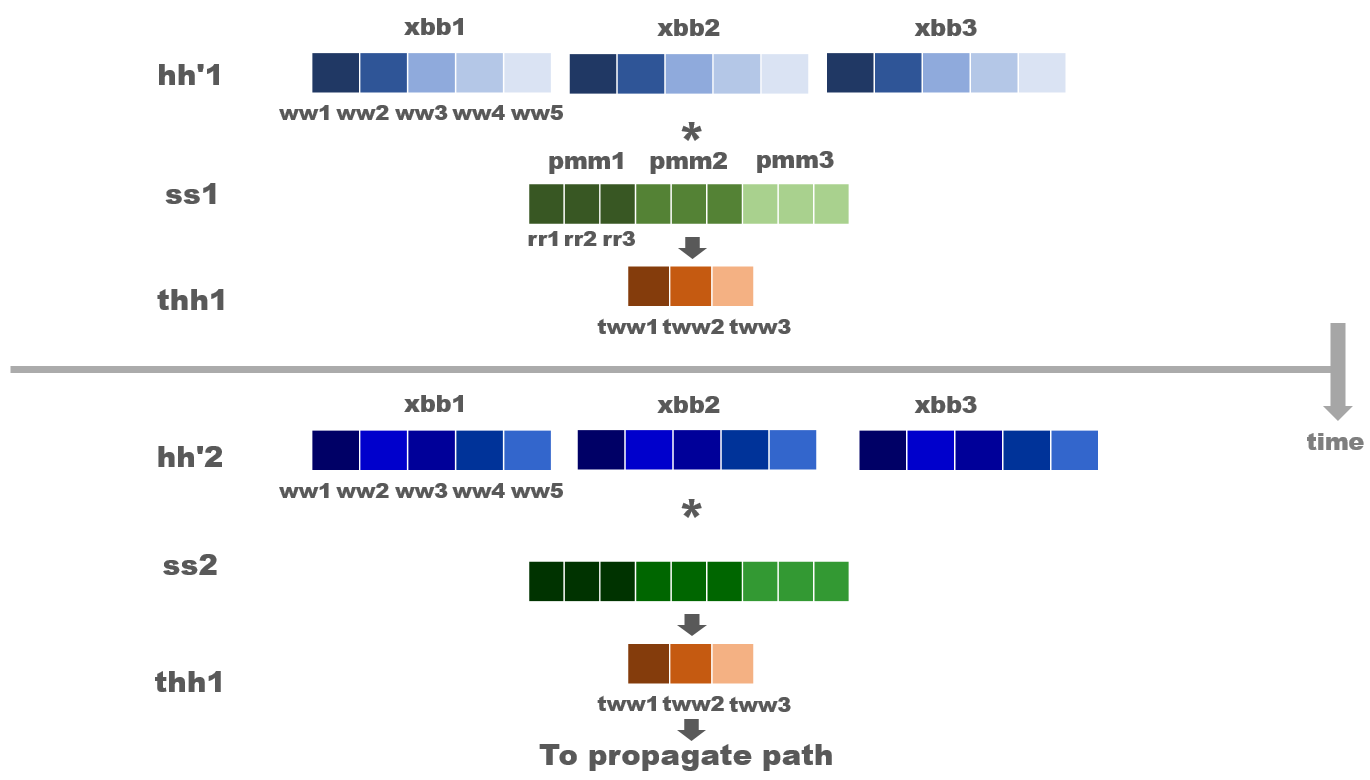
\includegraphics[width=1\linewidth]{inc/4_proposed_architecture/figure/xb_to_s.png}
    \caption{An example of 1D convolution with $T_w=3,X_b=3,S=2$ , at finishing first convolution row after 3 input bit channels, we proceed to second row convolution ss2, and then finish the output row thh1, sending partial sum out of PE.}
    \label{fig:xb_to_s}
\end{figure}
To be able to quantize and re-pack output data as soon as the partial sum is finished, a column of PEs need to process in lock-step. We then group a column of PEs as an unit, this gives us several opportunities for hardware sharing. The main controller is shared across a PE column, a main controller in a PE actually takes up about 5\% of area, if not shared, approximately an additional 54k gates area is needed for each column. Filter reuse along row in a PE column is a significant data reuse-ability, the input data from input pad is shared for every filters from different PE rows. We then put only one input pad in a PE column accordingly, this saves 360B of register file storage space in a PE column. Since PE array is of large 16-column, the mentioned resource sharing contributes hugely. 

\begin{table}[h] 
    \caption{PAD specifications}
    \label{tab:pad_spec}
    \centering
    \footnotesize 
        \begin{tabular}{c|ccc}
        \toprule
        PAD & size & width & total size (entire chip)\\
        \midrule
        Input &  12 & 16b & 384B\\
        Weight &  48 & 16b& 24KB\\
        Partial sum & 32 & 32b & 32KB\\
        \bottomrule
        \end{tabular}
\end{table}
\begin{table}[h]
    \caption{PAD constraints}
    \label{tab:pad_cons}
    \centering
    \footnotesize 
        \begin{tabular}{c|c}
        \toprule
        PAD &  constraints\\
        \midrule
        Input & $R*P_{ch} \leq 12$\\
        Weight & $R*P_m*P_{ch} \leq 48$\\
        Partial sum & $T_w*P_m*psum\ width \leq 64$ \\
        \bottomrule
        \multicolumn{2}{c}{psum width is either 1/2 word, a word is 16-bit}
        \end{tabular}
\end{table}


\subsection{Re-configurable arithmetic logic unit}
First we review the low-precision operation details. The input and weight data is re-packed along channel dimension based on arithmetic bit length $A_b$ into a data of 16-bit word. The channel dimension in CNN is meant to be accumulated together. \autoref{fig:mult_add} shows a 4x 4-bit multiplication and addition is needed for such data. Similarly, we need 16x MAC for 1-bit data, 8x for 2-bit, 2x for 8-bit. We call such basic operator \textbf{MAT} as in \textit{multiplier adder tree}, as it performs $16/A_b$ multiplications and sums them up. The multiplication needs to support either signed or unsigned mode. We also include \textit{XNOR} mode feature binarized layer as in \cite{XnorNet}, where each binary data 1 mapped to 1, 0 to -1. \\
\begin{figure}[h]
    \centering
    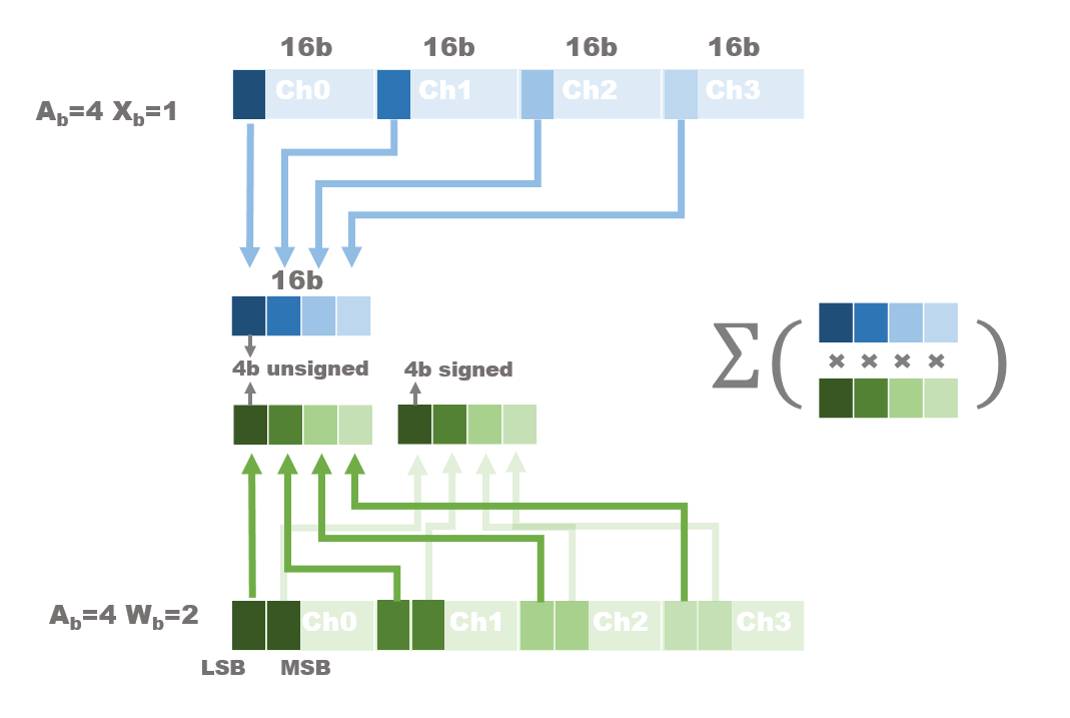
\includegraphics[width=1\linewidth]{inc/4_proposed_architecture/figure/mult_add.png}
    \caption{4-bit input and 8-bit weight re-packed using $A_b$=4.}
    \label{fig:mult_add}
\end{figure}
We propose three micro-architecture for such operations. The operators must support signed and unsigned 16x1b, 8x2b, 4x4b, 2x8b MAT and XNOR operation. The first one is 8-bit \textit{simple multiplication} MAT. The module takes an un-optimized multiplier as a base, masked out unused logics based on configuration, and add the 8 partial-product together for the final product. For XNOR mode, the partial product is replaced with XNOR gate rather than AND gate, then simply takes the 1-bit summation result \textbf{$P$}, which is essentially a bit-counting operation, and outputs $2*P-16$. Re-configurability on 5 modes with support of signed and unsigned data makes such design induces at least a 2-to-1 MUX on each bit of partial-product, as to be zero-gated, sign extended or the original partial-product. The routing cost is not to be overlooked, not to mention the long critical path of 8+8 ripple carry adder. The advantage of this design lies in no MUX for the final-product and the inputs. \\
\begin{figure}[h]
    \centering
    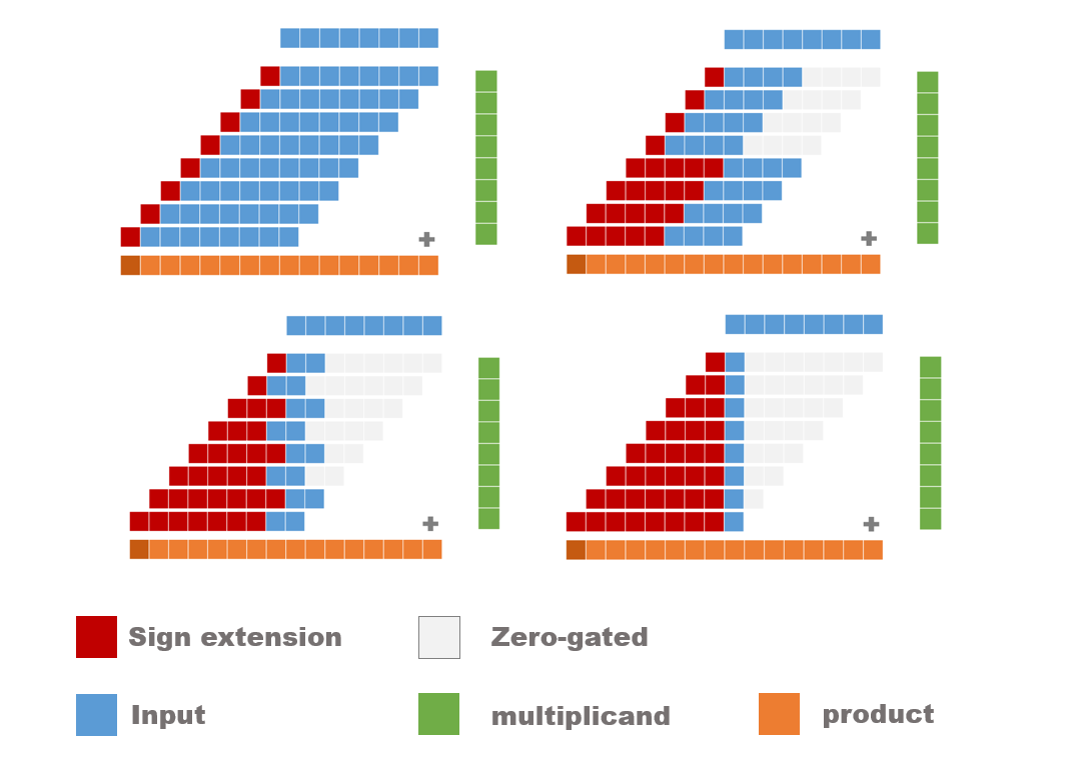
\includegraphics[width=0.8\linewidth]{inc/4_proposed_architecture/figure/simple_MAT.png}
    \caption{8,4,2,1-bit mode of simple MAT from upper-left to lower-right.}
    \label{fig:simple_MAT}
\end{figure}
\begin{figure}[t]
    \centering
    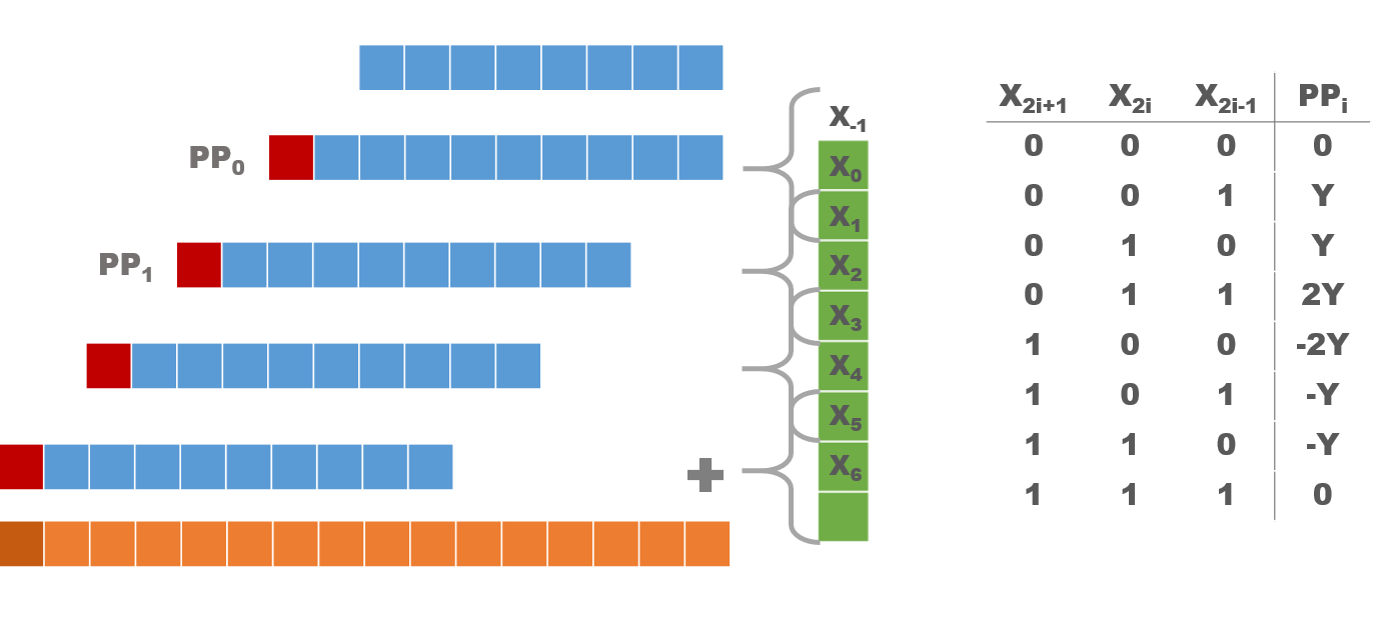
\includegraphics[width=0.8\linewidth]{inc/4_proposed_architecture/figure/booth_8.png}
    \caption{Partial product relation to 3 multiplicand bits in a group in a 8-bit signed booth multiplier.}
    \label{fig:booth_8}
\end{figure}
\begin{figure}[t]
    \centering
    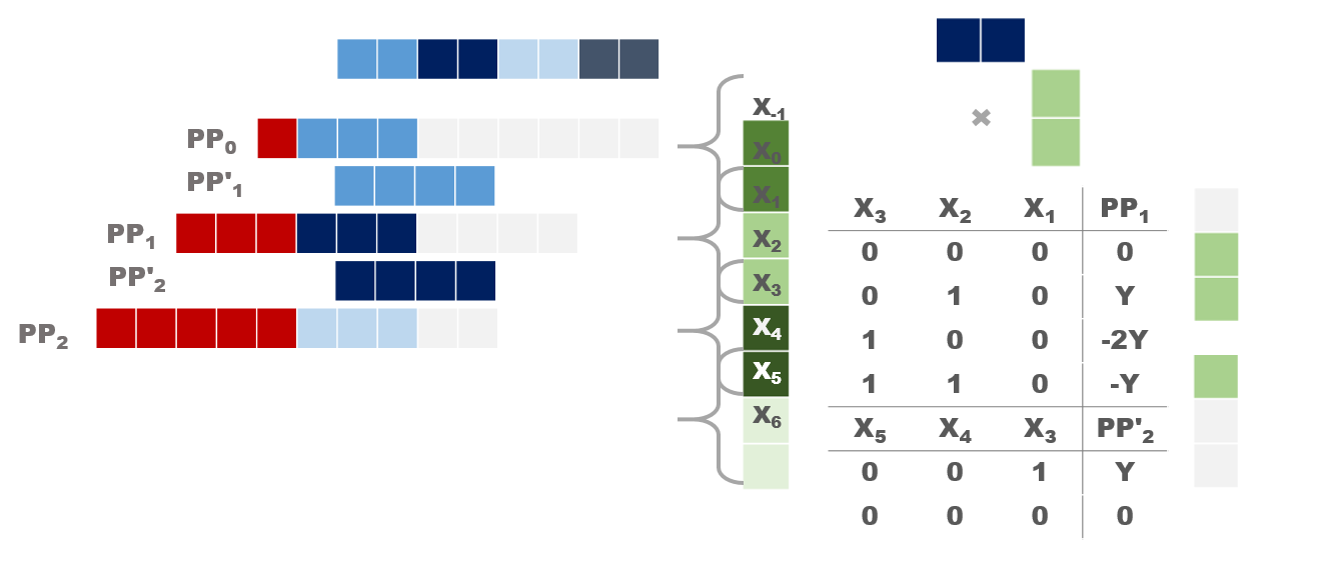
\includegraphics[width=0.8\linewidth]{inc/4_proposed_architecture/figure/booth_2b_on_8b.png}
    \caption{To perform 2-bit MAT on a 8-bit booth multiplier, the multiplicand will be properly zero-gated, the partial product has to carefully chosen, additional partial product needs to be added. }
    \label{fig:booth_2b_on_8b}
\end{figure}
\begin{figure}[t]
    \centering
    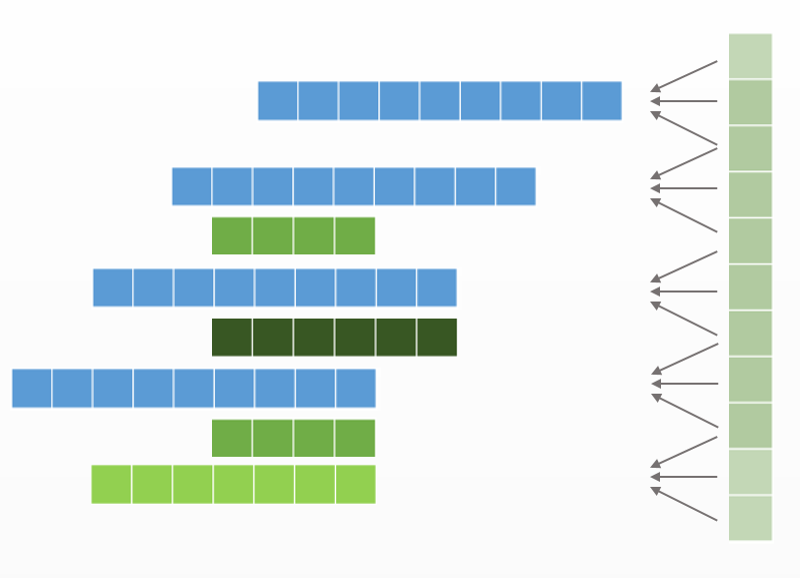
\includegraphics[width=0.8\linewidth]{inc/4_proposed_architecture/figure/booth_final.png}
    \caption{The additional partial product just for 2-bit and 1-bit configuration.}
    \label{fig:booth_final}
\end{figure}
The second one \textit{booth MAT} is based on booth-algorithm multiplier. A typical radix-4 signed booth multiplier reduced the partial-product from 8 down to 4. Radix-4 setting straight up implies no partial-product and critical path saving for 2-bit and 1-bit operations, since it produced a partial-product per 3-bit multiplicand (the weight or the green bits), larger than what 2-bit and 1-bit need. We have to add additional partial product for unsigned setting and 2-bit, 1-bit mode. The basic working principle is provided in \autoref{fig:booth_8}. To perform 2-bit or 1-bit MAT on a 8-bit booth multiplier, additional partial products and new multiplicand zero-gated rules are added. The reasoning can be developed from piecing together wanted 2-bit partial product, as in \autoref{fig:booth_2b_on_8b}, we need the two partial product shown in the right portion of the figure, so we need the two zero-gated 3-bit multiplicand and an additional partial product based on the gated multiplicand. In turn, the routing and MUX-ing in this design is unbearably complicated, so as the synthesis result show. The additional partial products needed is shown in \autoref{fig:booth_final}. \\
\begin{figure}[h!]
    \centering
    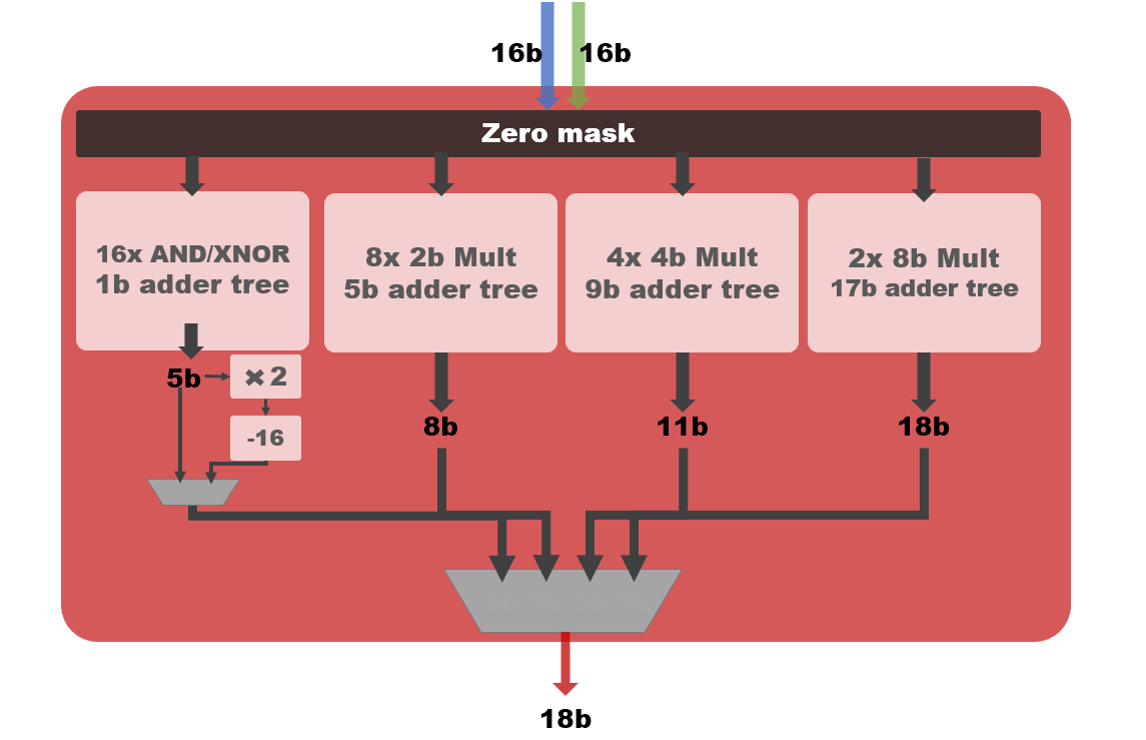
\includegraphics[width=0.9\linewidth]{inc/4_proposed_architecture/figure/MATmux.png}
    \caption{MATmux chooses the configured product as the output, masked out idle adder trees and multipliers.}
    \label{fig:MATmux}
\end{figure}
The last design \textit{Mux MAT} is the simplest yet the most efficient in every aspects. It takes in 16-bit input and weight, broadcasts both data to 4 set of multipliers and adder trees units, however zero-gated input port to the idle units. The multipliers and adder trees bits are chosen in order to support both signed and unsigned data by sign extending the product, that is 1,5,9,17-bit for 1,2,4,8 multiplication respectively. The output bits are chosen for the maximum required bit-length of the adder tree output. XNOR mode takes the XNORed gates bit-counting results, multiplies it by 2 and subtract 16. 

Synthesis results concludes for using MUX MAT design. For the time being, we focus on the slack where it determines the critical path of the system, it plays the most important role in low-power consumption goal. Simple mult design and booth both haven't met our desired constraint, so we did not do thorough verification on them, the synthesis area would possibly go up. 
\begin{table}
    \caption{Synthesis for MAT designs}
    \label{tab:pad_cons}
    \centering
    \footnotesize 
        \begin{tabular}{c|cc}
        \toprule
        Design &  cell area (TSMC 90nm) & slack (400MHz)\\
        \midrule
        simple multiplication & 11815* \footnotemark & 0\\
        booth & 9618* & 0\\
        MUX & 13659 & 0.30\\
        16b multiplication (32b output) & 11486 & 0**\\
        16b multiplication (16b output) & 4274 & 0**\footnotemark\\
        \bottomrule
        \end{tabular}

\end{table}
\footnotetext[1]{*correctness not checked}
\footnotetext{** typically 16-bit multiplication won't fit in a 2.5ns cycle time even on 65nm process}
\begin{figure}[h]
    \centering
    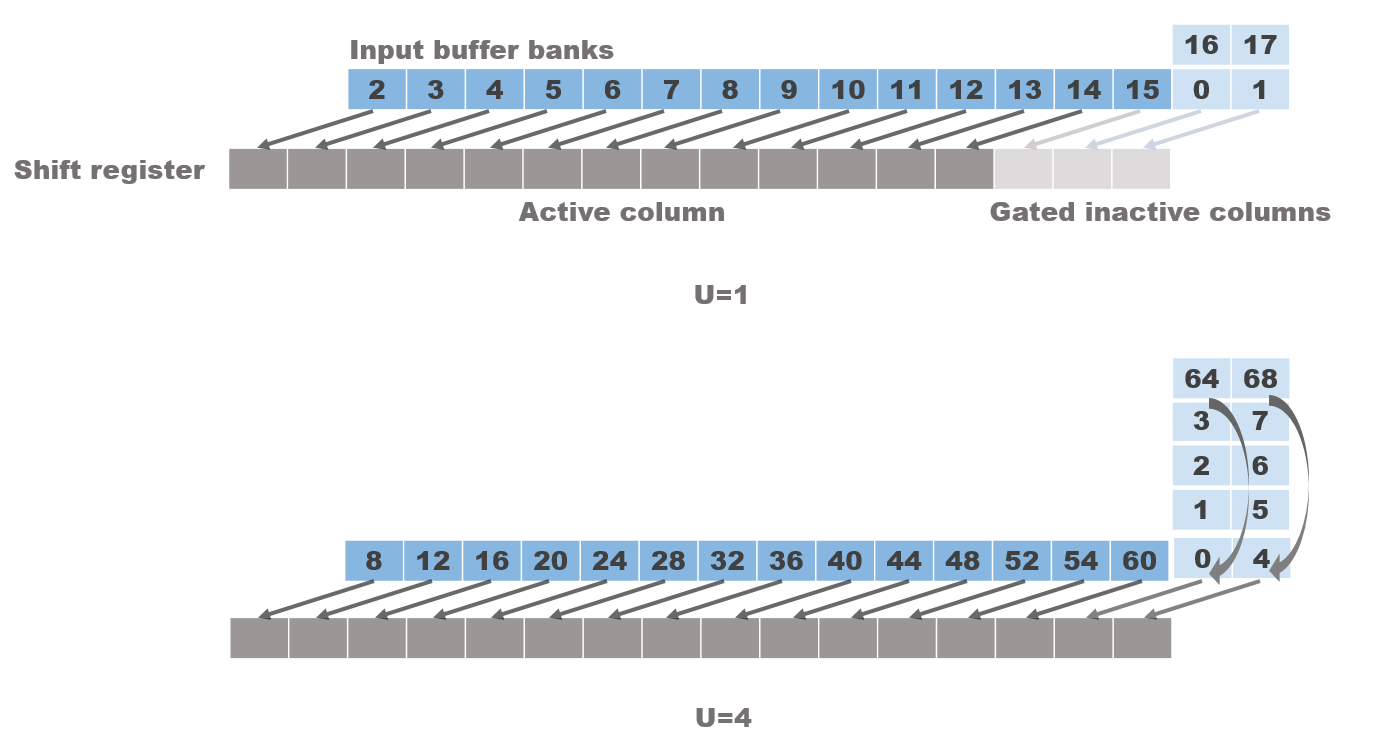
\includegraphics[width=1\linewidth]{inc/4_proposed_architecture/figure/shift.png}
    \caption{Following previous example, each PE column access needed data simultaneously, the bandwidth is not wasted.}
    \label{fig:shift_dispatcher}
\end{figure}
\subsection{Shift dispatcher}
Shift dispatcher between buffers and PE array are just a circular shift-register. As the input is re-arranged based on stride $U$ either off-line (first layer) or naturally aligned by the processing of the system at the output, every PE columns can access required data from each input banks at the same cycle. The registers are gated if corresponding PE column is inactive. \autoref{fig:shift_dispatcher} demonstrate a $U=1,S=3,ss=3$ and a $U=4,S=11,ss=9$ example where left shift 2 is needed for both.  

\subsection{Quantization}
We use round to the nearest quantization scheme. After the final scaling and shifting, we save two digit behind the decimal point, in other word we right shift $\gamma'=gamma-2$ 2 less digit than the real shifting factor. Now for positive number, the result add 1 if the first digit behind decimal point is 1, otherwise get rid all the decimals. For negative number, the result add 1 if the two digits behind decimal point is $11$, otherwise get rid of all the decimals. For example a positive number $01000.1_b$ is rounded to $01001$, that is 8.5 rounded to 9; a negative number $10111.11_b$ is rounded to $11000$, that is -8.25 rounded to -8. 

\iffalse
\TODO{final choice}.
\textcolor{purple}{This chapter is your proof. You have shown in the previous chapters what the starting point is and why it is important to advance. This chapter describes how you advance and how you made choices. It also shows what (performance) results your choices lead to. Ideally, it identifies how certain choices influence the final performance.}
\fi